\chapter{Resultados Obtidos}

Para validar o sistema, é preciso testar e botar a prova os requisitos mecânicos, de custo, e de desempenho do aplicativo. 

\section{Requisitos Mecânicos}

A plataforma fabricada totalizou xg sem o Ball Head da câmera. A tabela \ref{} discrimina o peso de cada componente. Mas, mesmo leve, mostrou-se limitada em suportar lentes pesadas pois, ao longo dos inúmeros testes de campo com a plataforma, a engrenagem impressa que é acoplada no motor rachou. 

\subsection{Impressão 3D}
A engrenagem menor é o elo mais fraco no sistema de transmissão, isso se deve pelo seu tamanho mais reduzido. A primeira versão da impressão 3D acabou sofrendo um rachamento em função de não suportar o torque do motor. Na Figura \ref{} é possível verificar que o furo se forma no plano de contato entre as engrenagens, tornando mais evidente o motivo da ruptura.

Além disso, quando a engrenagem apresentou a rachadura, o peso do sistema totalizava 2,5kg com ball head x, câmera X e lente X. Este acontecimento não invalida o projeto pois ocorreu com um peso de rastreamento superior à meta proposta, e, por isso, recomenda-se cautela em situações onde o equipamento se aproxima ou ultrapassa a marca de 2,5kg de peso total. 

 

\subsection{Eixo Curvado}

O Eixo curvado não têm sua curvatura montada de forma ideal. A Figura \ref{} torna claro a discrepância entre como deveria ser, e como ficou. Esse erro de fabricação gerou inconsistência em certos pontos no funcionamento da plataforma, e eles serão demonstrados na próxima seção.

\subsection{Análise de Consistência}
A velocidade e vibração da plataforma foram analisados por meio de um sensor acelerômetro instalado na plataforma como demonstra a Figura \ref{}. Com esses testes, foi possível comparar diferentes cenários de uso de elementos amortecedores no sistema e o seu impacto na consistência e vibração. Os dados foram obtidos em uma taxa de 100Hz utilizando um arduíno e comunicação Serial com um notebook que armazenava os dados. 

...



\section{Custo Total do Sistema}
O custo dos materiais e processos de fabricação estão descritos na tabela \ref{}, com a qual pode se constar um total de x reais envolvendo materiais e fabricação de componentes. Comparando ao valor do NyxTech -- que possui uma construção e materiais similares, com um preço de US\$ 110 -- o EasyTracker conseguiu vencer a meta de custo.  

\section{Análise de Desempenho do Aplicativo}
O Software pode ser avaliado com relação ao uso e implementação das heurísticas de desenvolvimento, com relação ao desempenho em hardware -- consumo de processamento e memória --, e ainda pode ser avaliada com Feedbacks dos usuários. 

\subsection{Interface Gráfica}
Quando à interface e recursos, é possível avaliar de forma qualitativa como as 10 Heurísticas de Nielsen foram utilizadas. Os status cruciais para funcionamento são todos visíveis: o status \textit{bluetooth} do sistema é visível por meio do estado do botão de conexão na tela de visualização do perfil. Nas telas de alinhamento, se o sistema está alinhado, os ícones ficam esverdeados, caso contrário ficam avermelhados.

Além disso, as cores e os elementos de ícones são similares com o que os usuários estão acostumados, como os ícones nas telas de perfis de localização que fazem sentido para o contexto e são minimalistas. Além disso, as telas de alinhamento se assemelha a uma bolha de nível onde o acelerômetro é empregado. Na tela de alinhamento com o polo magnético, o sistema emula uma bússola. 

Nessas mesmas telas de alinhamento, os usuários podem controlar livremente o fluxo das telas de alinhamento. Dessa forma conseguem conferir alguma informação que possam ter deixado passar, assim como podem navegar para telas de ajudas e retornar.

Não obstante, a consistência desses padrões nas telas de alinhamento também foram consolidado nas telas de perfis. As ações de criar, editar, e visualizar um perfil usam por base a mesma tela, facilitando para o usuário entender o que ocorre no sistema. 

Além disso, a prevenção de erros é feita de forma ativa relembrando o usuário de, por exemplo, recomendando uma calibração da bússola ao entrar na tela de alinhamento azimutal, ou também com um popup para atualizar os dados de declinação magnética em localizações que foram armazenadas a mais e 2 meses. A prevenção também ocorre nas entradas de dados:  onde o usuário precisa inserir valores de latitude e declinação, que devem ser valores decimais. No entanto, eles podem ser escritos em graus, minutos e segundos, mas o usuário não vai conseguir inserir dessa forma, pois, o teclado numérico não permite essa formatação.

\begin{figure}[!htb]
	\centering
	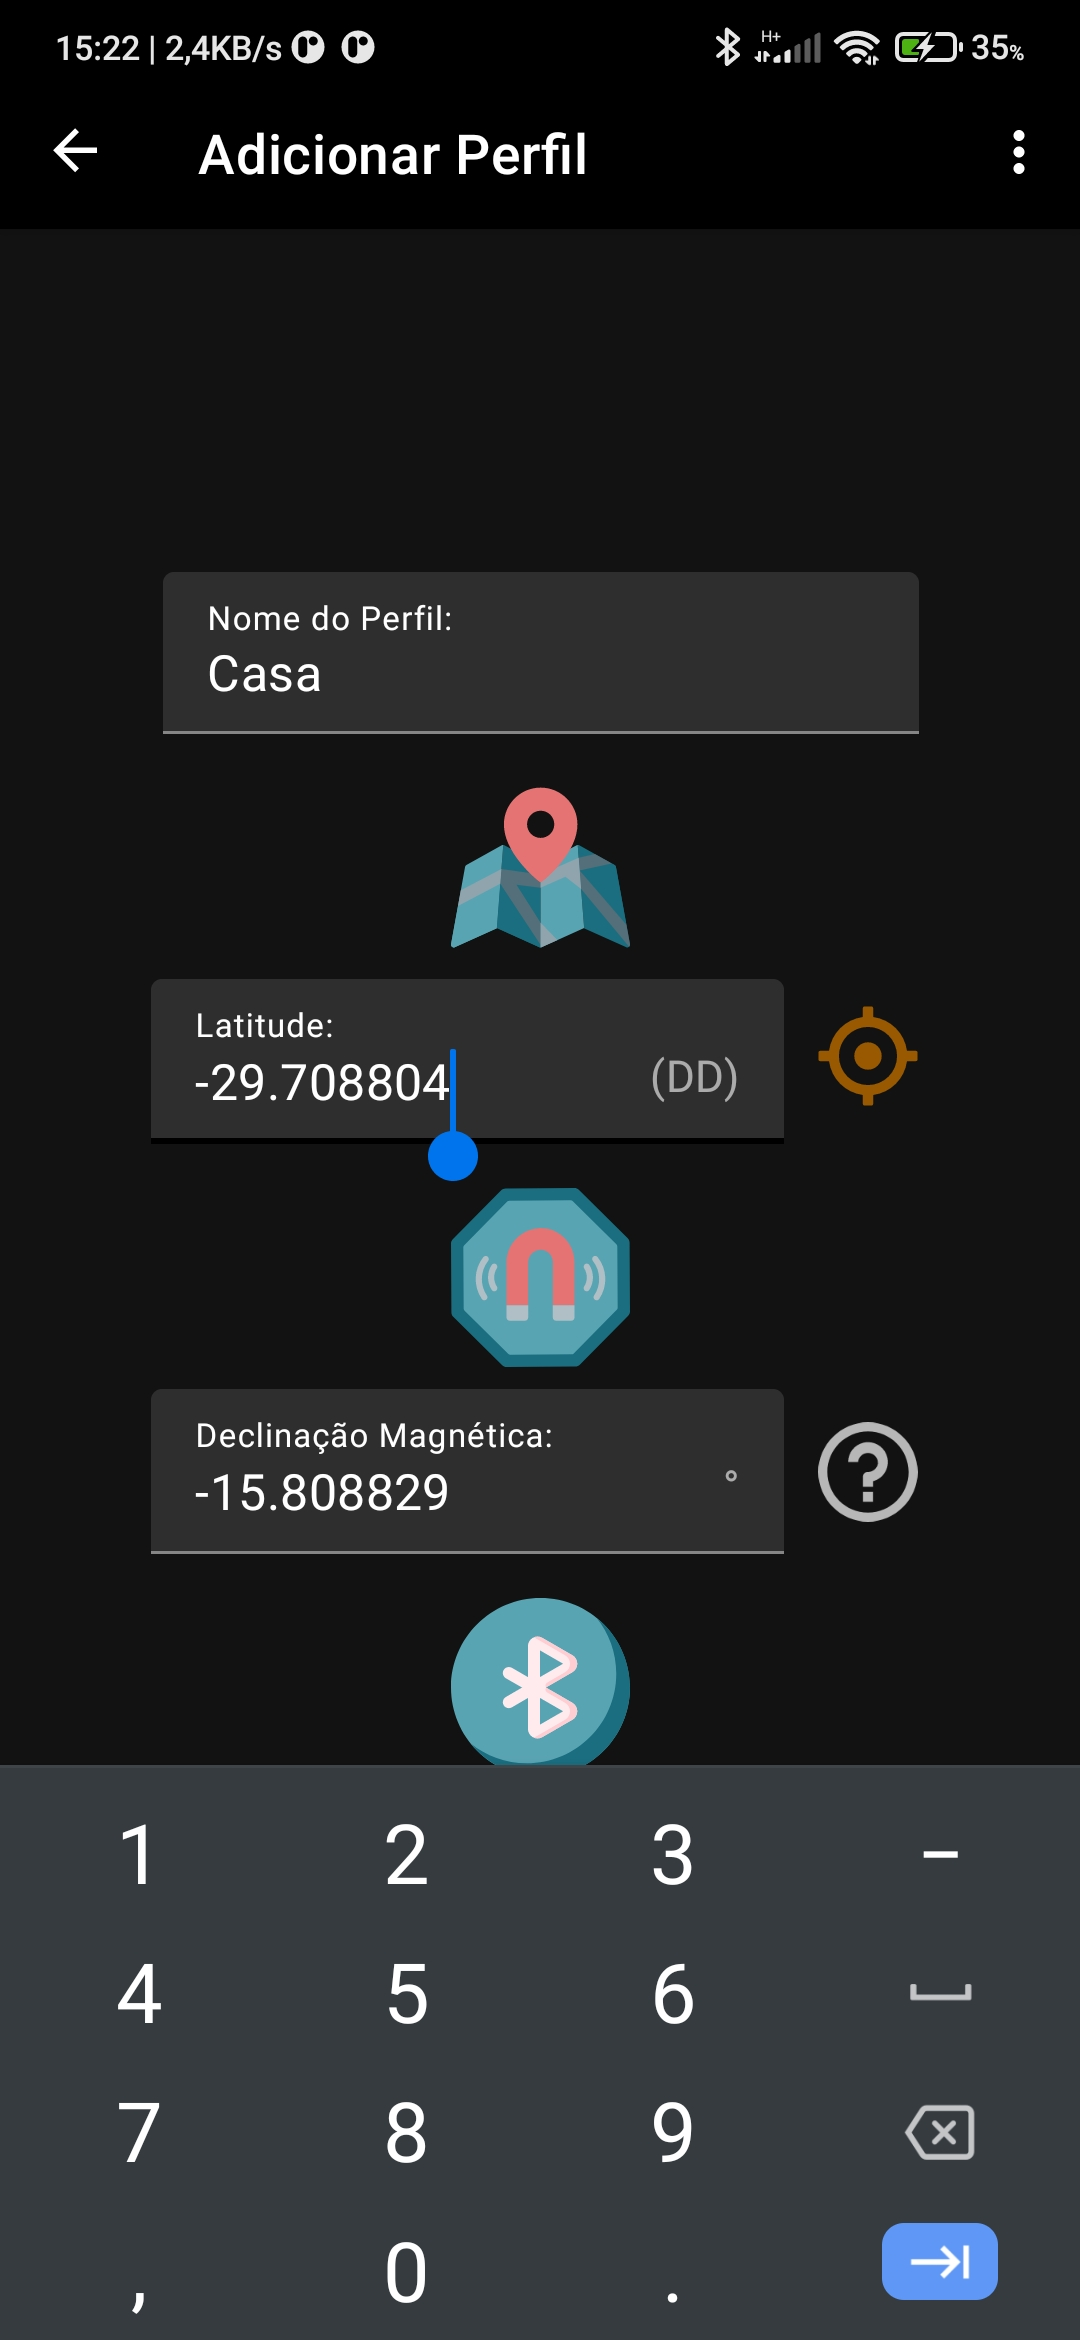
\includegraphics[width=0.3\linewidth]{figuras/resultados/gpsedit}
	\caption{Teclado só permite uso de vírgula e ponto, não permitindo aspas e sinal de grau $ (^\circ) $}
	\label{fig:gpsedit}
\end{figure}

Por fim, uma seção de perguntas e respostas básicas foi implementada. É uma lista de perguntas que funcionam com efeito de sanfona para mostrar as respostas. No entanto, o princípio de customização não foi implementado ainda. Sugere-se essa implementação nos trabalhos futuros, com uma tela de configuração do aplicativo. 

Dessa forma, o desenvolvimento da interface gráfica do aplicativo conseguiu atingir um estágio de desenvolvimento compatível com o estado da arte atual relativo a criação de aplicativos Android ou outros Softwares. As heurísticas foram respeitadas e a implementação é fluída, os itens estão dispostos respeitando uma hierarquia visual que está em conluio com a identidade do projeto e os recursos do Android. 

\subsection{Desempenho}
O aplicativo foi desenvolvido e testado em 2 dispositivos, celular Xiaomi Mi 9 Lite\footnote{especificações} e tablet Multilaser M10 Lite\footnote{especificações}.Com o emulador do Andorid Studio, foi possível simular outros dispositivos com telas de tamanhos variados, garantindo que os itens foram dispostos de maneira inteligente, e conseguem se adaptar aos mais diversos celulares. 

No Mi 9 Lite, foi possível averiguar uma boa resposta na interface, com um consumo de até 250mb de memória RAM e 20\% de processamento, atingindo este pico quando o aplicativo está nas telas de alinhamento. Para o tablet...

Portanto...
buscar referencias para erificar desempenho


\section{Fotografias}